\subsection{State diagram}

\begin{figure}[h]
\centering
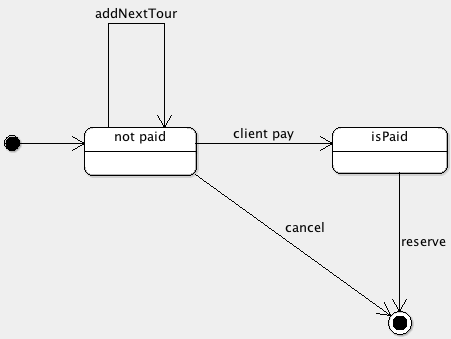
\includegraphics[width=8cm]{project/images/state.png}
\caption{State diagram}
\end{figure}

\paragraph{}
After created, the reservation of touring travel have two middle states: \textit{isPaid}, and \textit{notPaid}. When in \textit{notPaid}, we can add as many more tour as we can, or if we cancel the reservation, it will fall into final state. When the client pay for the reservation, object's state will change into \textit{isPaid}, and no more modification could be done. And when the reservation for flight, hotel, car were done, it will come to final state.